\documentclass[12pt]{article}

\usepackage[utf8]{inputenc}
\usepackage{amsmath,amsthm,amsfonts,amssymb,amscd}
\usepackage{multirow,booktabs}
\usepackage[table]{xcolor}
\usepackage{fullpage}
\usepackage{lastpage}
\usepackage{enumitem}
\usepackage{fancyhdr}
\usepackage{mathrsfs}
\usepackage{wrapfig}
\usepackage{setspace}
\usepackage{calc}
\usepackage{multicol}
\usepackage{cancel}

\usepackage{graphicx}
%%\usepackage{caption}
%%\usepackage{subcaption}


\usepackage{listings}
\usepackage{matlab-prettifier}
\usepackage[framed,numbered,autolinebreaks,useliterate]{mcode}

\usepackage[margin=3cm]{geometry}
\newlength{\tabcont}
\setlength{\parindent}{0.0in}
\setlength{\parskip}{0.05in}
\usepackage{empheq}
\usepackage{framed}
\usepackage[most]{tcolorbox}
\usepackage{xcolor}
\colorlet{shadecolor}{orange!15}
\parindent 0in
\parskip 12pt
\geometry{margin=1in, headsep=0.25in}
\usepackage{float}
\usepackage{graphicx}
\usepackage{hyperref}


\newtheorem{thm}{Theorem}
\theoremstyle{theorem}
\newtheorem{reg}{Rule}
\newtheorem{exe}{Exercise}
\newtheorem{rem}{Remark}
\newtheorem{cor}{Corollary}
\newtheorem{exa}{Example}
\newtheorem{defi}{Definition}

\usepackage{natbib}
\bibliographystyle{abbrv}

\usepackage{times}
%\usepackage[compact]{titlesec}
\usepackage{titlesec}
\titlespacing*{\section}{0pt}{*-2}{*-1}
\titlespacing*{\subsection}{0pt}{*-2}{*-1}
\titlespacing*{\subsubsection}{0pt}{*-2}{*-1}

\def\a{\alpha}
\def\b{\beta}
\def\de{\delta}
\def\De{\Delta}
\def\ga{\gamma}
\def\Si{\Sigma}
\def\si{\sigma}
\def\ep{\varepsilon}
\def\ze{\zeta}
\def\om{\omega}
\def\leq{\leqslant}
\def\rar{\rightarrow}
\def\Rar{\Rightarrow}
\def\td{\Leftrightarrow}
\def\R{\hro{R}}
\def\C{\hro{C}}
\def\hro{\mathbb}
\def\bbI{\hro{I}}
\def\N{\hro{N}}
\def\Z{\hro{Z}}

\def\tE{\tilde{E}}
\def\hE{\hat{E}}
\def\tA{\tilde{A}}
\def\tT{\tilde{T}}
\def\hA{\hat{A}}
\def\hD{\hat{D}}
\def\bA{\breve{A}}
\def\tB{\tilde{B}}
\def\hB{\hat{B}}
\def\tC{\tilde{C}}
\def\tN{\tilde{N}}
\def\hN{\hat{N}}
\def\tk{\tilde{k}}
\def\tX{\tilde{X}}
\def\hX{\hat{X}}
\def\bX{\breve{X}}
\def\tM{\tilde{M}}
\def\tm{\tilde{m}}
\def\bM{\breve{M}}
\def\hM{\hat{M}}
\def\bm{\breve{m}}
\def\tH{\tilde{H}}
\def\tF{\tilde{F}}
\def\tG{\tilde{G}}
\def\hG{\hat{G}}
\def\tK{\tilde{K}}
\def\tx{\tilde{x}}
\def\tf{\tilde{f}}
\def\hf{\hat{f}}
\def\brf{\breve{f}}
\def\baf{\bar{f}}
\def\tg{\tilde{g}}
\def\hg{\hat{g}}
\def\lb{\lambda}
\def\cP{{\cal P}}
\def\cQ{{\cal Q}}
\def\fr{\frac}
\def\frQ{\mathfrak{Q}}

\def\cU{{\cal U}}
\def\cV{{\cal V}}
\def\cH{{\cal H}}
\def\tcU{{\tilde{\cal U}}}
\def\cZ{{\cal Z}}

\def\hxi{\widehat{\xi}}
\def\hp{\hat{q}}

\def\ddt{\fr{\mathrm{d}}{\mathrm{d}t}}
\def\dtau{\Delta_{\tau}}
\def\tnu{\tilde{\nu}}
\def\tU{\tilde{U}}

\def\tcQ{{\tilde{\cal Q}}}
\def\tcP{{\tilde{\cal P}}}
\def\hcP{\widehat{\cP}}
\def\hcQ{\widehat{\cQ}}
\def\cE{\mathcal{E}}
\def\cA{\mathcal{A}}
\def\cD{\mathcal{D}}
\def\hcE{\hat{\cE}}
\def\hcA{\hat{\cA}}
\def\hcD{\hat{\cD}}
\def\vphi{\varphi}

\newcommand{\n}[1]{\left\lVert#1\right\rVert}

\newcommand{\m}[1]{
	\begin{bmatrix}
		#1
	\end{bmatrix}
}

\renewcommand{\pm}[1]{
	\begin{matrix}
		#1
	\end{matrix}
}

\def\ES{
	\begin{bmatrix}
		J^E  & 0        & 0       & 0 \\
		0       & N^E_{2} & 0       & 0 \\
		0       & 0        & N^E_{3}& 0 \\
		0       & 0        & 0       & N^E_{4} 
	\end{bmatrix}
}

\def\AS{
	\begin{bmatrix}
		A_{1}  & 0       & 0          &  0        \\
		0           & J^A  & 0          & 0      \\
		0           &   0                & N^A_{3}      & 0      \\
		0           &   0                & 0                    & N^A_{4}      
	\end{bmatrix}
}
\def\BS{
	\begin{bmatrix}
		B_{1}  & 0       & 0        & 0 \\
		0          & B_{2}       & 0        & 0 \\
		0          & 0                  & J^B  & 0  \\
		0          & 0                 &   0                & N^B_{4}  \\ 
	\end{bmatrix}
}

\def\be{\begin{equation}}
\def\ee{\end{equation}}         

\newcommand{\ben}{\begin{eqnarray}}
\newcommand{\een}{\end{eqnarray}}

\newcommand{\bens}{\begin{eqnarray*}}
\newcommand{\eens}{\end{eqnarray*}}

\def\bc{\begin{cases}}
\def\ec{\end{cases}}

\newcommand{\bsq}{\begin{subequations}}
\newcommand{\esq}{\end{subequations}}

\newcommand{\eproof}{\space
	{\ \vbox{\hrule\hbox{\vrule height1.3ex\hskip0.8ex\vrule}\hrule}}\\[0.2cm]}

\begin{document}
% \setcounter{section}{8} This is assumed that count from Section 9

\thispagestyle{empty}

\begin{center}
	{\LARGE \bf Chapter 5. Best Approximation in $C[a,b]$ \\ Least square approximation}\\[.2cm]
	{\large Numerical Analysis 1. Winter Semester 2018-19}
\end{center}

\section{Best Approximation in $C[a,b]$}

Let $f(x)$ be a given function that is continuous on some interval $[a,b]$. If $p(x)$ is an interpolation polynomial, then we are interested in measuring 
%
\[  
\min_{\deg p\leq n} E(p) := \min_{\deg p\leq n} \max_{a\leq x\leq b} |f(x)-p(x)| \ .
\]
%
\begin{shaded}
\textbf{Chebyshev polynomials} \ For $x \in [-1,1]$, define $T_n(x) = \cos[n \arccos x]$, for each $n \geq 0$. \\
\textbf{Three term recurrence}
\[ T_{n+1}(x) = 2x T_{n} - T_{n-1} \ . \]
\textbf{Monic Chebyshev polynomials} 
\[ \tilde{T}_n(x) =  \dfrac{T_n(x)}{2^n} \ .\]
\end{shaded}

\begin{figure}[h!]
	\centering
	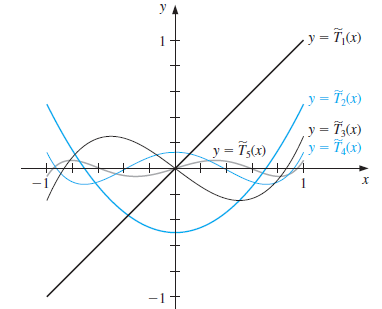
\includegraphics[scale = 0.9]{Figures/30}
\end{figure}

\begin{thm}
The Chebyshev polynomial $T_n(x)$ of degree $n \geq 1$ has $n$ simple zeros in $[-1, 1]$ at
%
\[ x_k = \cos \big( \frac{2k-1}{2n} \pi \big), \mbox{ for each } k = 1, 2, \dots , n. \]
%
Moreover, $T_n(x)$ assumes its absolute extrema at $x_k'=\cos \big(\frac{k\pi}{n}\big)$ with $T_n(x_k') = (-1)^k$, for each $k = 0, 1,\dots,n$.\\
\end{thm}

Let $\widetilde{\prod}_n$ denote the set of all monic polynomials of degree n.
\begin{thm}
The polynomials of the form $\tT_n(x)$, when $n \geq 1$, have the property that
\[ \frac{1}{2n-1} = \underset{x \in [-1,1]}{\max}|\tT_n(x)| \leq  \underset{x \in [-1,1]}{\max} |P_n(x)|, \mbox{ for all } P_n(x) \in \widetilde{\prod}_n \ .
 \]
Moreover, equality can occur only if $P_n = \tT_n$.
\end{thm}

Why are the Chebyshev nodes generally better than equally spaced nodes in polynomial interpolation? The answer lies in the term $\prod_{i=0}^{n}(x-x_i)$ that occurs in the error formula. \linebreak If $x_i = \cos[(2i + 1)\pi/(2n + 2)]$, then
%
\begin{equation*}
 \prod_{i=0}^{n}(x-x_i) \leq \cfrac{1}{2^n} \mbox{ for all } x\in [-1,1].
\end{equation*}
% 

\subsection{Error estimation}

\begin{shaded}
\begin{cor}
If $P(x)$ is the interpolating polynomial of degree at most $n$ with nodes at the roots of $T_{n+1}(x)$, then
%
\[  \underset{x \in [-1,1]}{\max} |f(x)-P(x)| \leq \cfrac{1}{2n(n + 1)!} \ \underset{x \in [-1,1]}{\max} | f^{(n+1)}(x)|, \mbox{ for each } f \in C^{n+1}[-1,1] \ . \]%
\end{cor}
\end{shaded}

\cleardoublepage 

\section{Approximation in the least square sense}

\subsection{Discrete time case: Least Square Approximation Using Data Table}

The wonderfully written motivation for least square approximation can be found from page 482-486, \cite{BurF10}.
\begin{center}
\begin{tabular}[12]{l|l|l|l|l|l|l|l|l|l|l}
X & 1 & 2 & 3 & 4 & 5 & 6 & 7 & 8 & 9 & 10 \\ \hline 	
Y & 1.3 & 3.5 & 4.2 & 5.0 & 7.0 & 8.8 & 10.1 & 12.5 & 13.0 & 15.6
\end{tabular}	
\end{center}

\begin{figure}[h!]
	\centering
	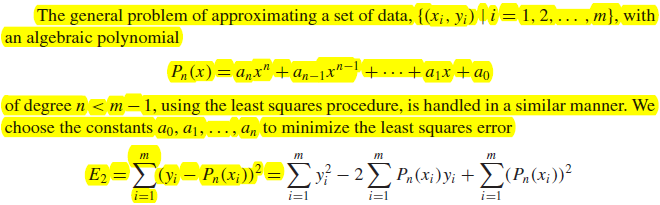
\includegraphics[scale = 0.8]{Figures/32}	
\end{figure}

\begin{figure}[h!]
	\centering
	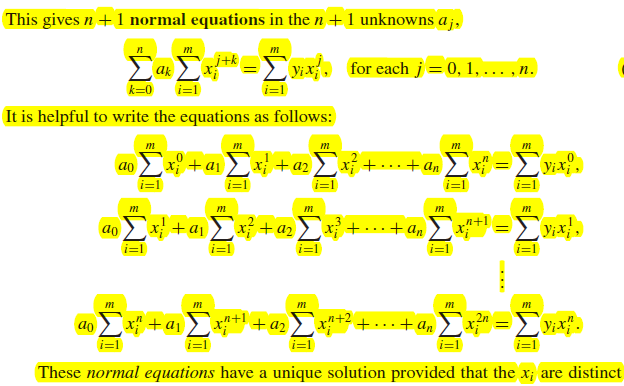
\includegraphics[scale = 0.8]{Figures/33}
\end{figure}

\begin{shaded}
1.	The \emph{least squares approximation (discrete time)} is the solution $\vec{a}$ to the \textbf{normal system} $A \vec{a} = b$, where
	%
	\begin{equation*}
	A = [a_{ij}], \quad a_{ij} = <P_i(X),P_j(X)>, \quad b_j = <Y,P_j> \ .
	\end{equation*}  
	%
2.	In case of orthorgonal vectors $\{P_i(X), \ i=0,\dots,n\}$, the solution is 
    %
    \[ \vec{a}_j = \cfrac{b_j}{a_{jj}} = \cfrac{<Y,P_j>}{<P_i(X),P_j(X)>} \ . \]
	%
\end{shaded}

\subsection{Singular Value Decomposition (SVD) and Moore-Penrose Pseudo Inverse}

\begin{figure}[h!]
	\centering
	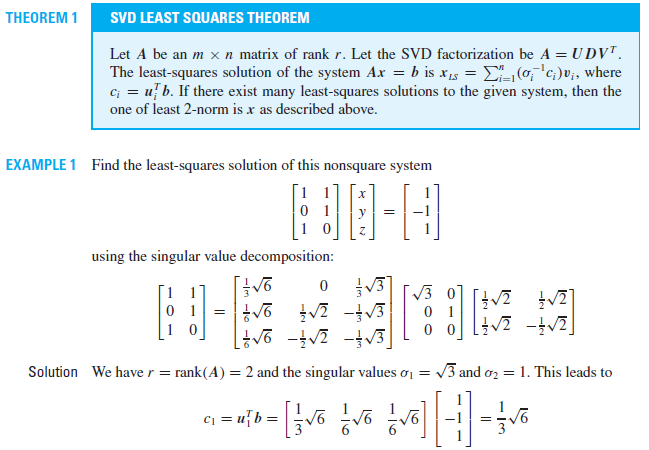
\includegraphics[scale  = 0.7]{Figures/41}
\end{figure}

\begin{figure}[h!]
	\centering
	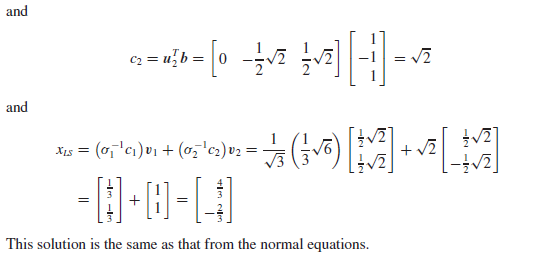
\includegraphics[scale  = 0.7]{Figures/42}
\end{figure}

\begin{figure}[h!]
	\centering
	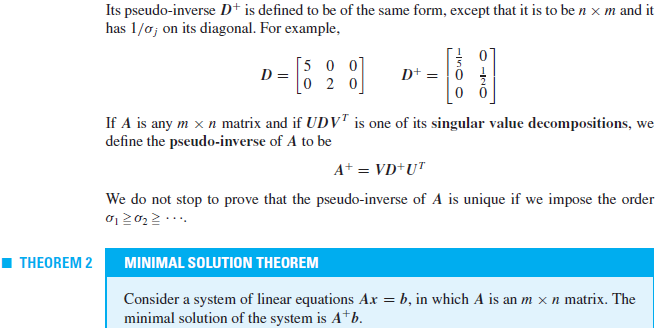
\includegraphics[scale  = 0.7]{Figures/43}
\end{figure}

\cleardoublepage 

\subsection{Continuous time case: Least Square Approximation $L_2[a,b]$}

The previous section considered the problem of least squares approximation to fit a collection of data. The other approximation problem mentioned in the introduction concerns the
approximation of functions.

\begin{figure}[h!]
	\centering
	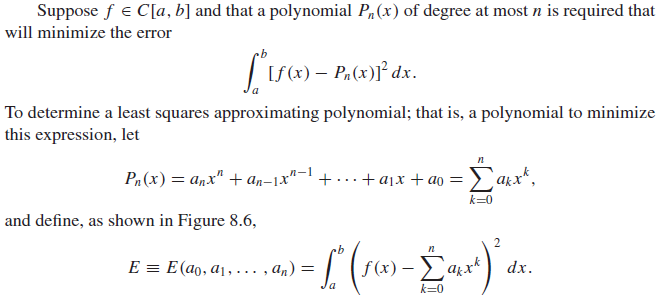
\includegraphics[scale  = 0.8]{Figures/34}
\end{figure}

\begin{figure}[h!]
	\centering
	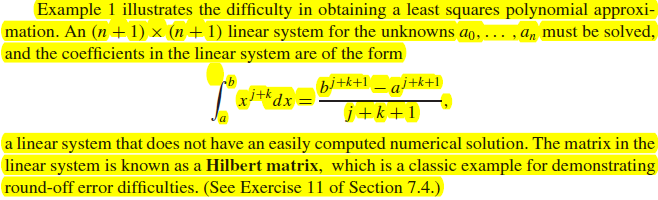
\includegraphics[scale = 0.8]{Figures/35}
	\label{fig:35}
\end{figure}

\begin{defi} An integrable function $w$ is called a \textbf{weight function} on the interval $\bbI$ if $w(x) \geq 0$, for all $x$ in $\bbI$, but $w(x) \not= 0$ on any subinterval of $\bbI$.
\end{defi}

The purpose of a weight function is to assign varying degrees of importance to approximations on certain portions of the interval. For example, the weight function	
places less emphasis near the center of the interval $(-1,1)$ and more emphasis when $|x|$ is near $1$.
\cleardoublepage 

\begin{figure}[h!]
	\centering
	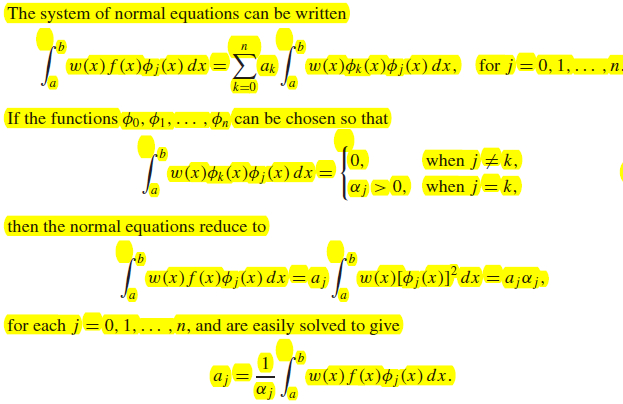
\includegraphics[scale = 0.8]{Figures/37}
	\label{fig:37}
\end{figure}

\begin{figure}[h!]
	\centering
	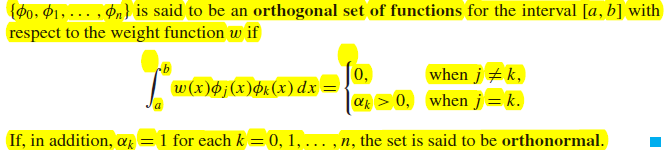
\includegraphics[scale = 0.8]{Figures/36}
	\caption{\cite{BurF10}, p. 499}
	\label{fig:36}
\end{figure}

\subsubsection{The Legendre polynomials} They have many special properties, and they are widely used in numerical analysis and applied mathematics. 

\begin{figure}[h!]
	\centering
	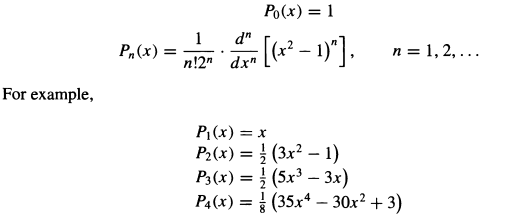
\includegraphics[scale = 0.8]{Figures/38}
	\caption{\cite{AtkH03}, p. 181}
	\label{fig:38}
\end{figure}

\begin{figure}[h!]
	\centering
	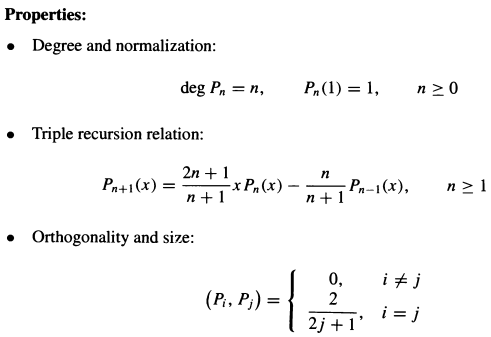
\includegraphics[scale = 0.8]{Figures/39}
	\label{fig:39}
\end{figure}

\begin{figure}[h!]
	\centering
	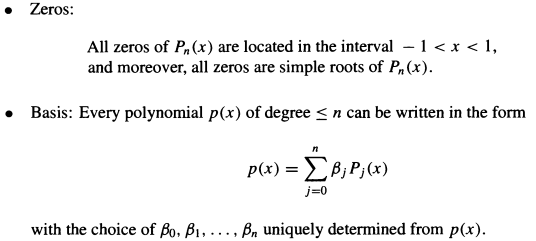
\includegraphics[scale = 0.8]{Figures/40}
	\label{fig:40}
\end{figure}

\begin{shaded}
The \emph{least squares approximation (continuous time)} of degree $n$ to $f(x)$ on $[-1,1]$ is
%
\begin{equation}\label{1}
 \ell_n(x) = \sum_{j=0}^{n} \cfrac{<f,P_j>}{<P_j,P_j>} P_j(x) \ .
\end{equation}  
%
\end{shaded}

\subsubsection{Least Squares Approximation with Weight}

For various reasons, we generalize the concept of “average error” by considering the so-called \emph{weighted least squares approximation}. 
%
\begin{equation*}
 \min\frac{1}{c} \int_{a}^{b} w(x) [f(x)-p(x)]^2 dx, \quad c=\int_{a}^{b} w(x)dx \ .
\end{equation*}
%
The function $w(x)$ is assumed to satisfy the following assumptions: 
\begin{enumerate}
\item[i.] $w(x)>0$ for alll $x\in  [a,b]$.
\item[ii.] For all integer $n$, $\int_{a}^{b} w(x) |x|^n dx < \infty$.
\end{enumerate}

With these assumptions, formula \eqref{1} is still valid, with the new scalar product 
%
\[  <f,g> := \int_{a}^{b} w(x) f(x) g(x) dx \ . 
 \]
%

\begin{exa}
The Chebyshev polynomial $\{T_n(x)\}$ are orthogonal on $(-1, 1)$ w.r.t. the weight function $w(x) = \cfrac{1}{\sqrt{1-x^2}}$ \ .
\end{exa}

\section{What have not been covered?}

\begin{shaded}
In this script we have not considered the following topics.
\begin{enumerate}
 \item[i)] Rational Function Approximation, see \cite{BurF10}, Section 8.4. 
 \item[ii)] Trigonometric Polynomial Approximation, see \cite{BurF10}, Section 8.5. 
\end{enumerate}
\end{shaded}

\section{Survey of Methods and Software}
In this chapter we considered approximating data and functions with elementary functions.
The elementary functions used were polynomials, rational functions, and trigonometric
polynomials. We considered two types of approximations, discrete and continuous. Discrete
approximations arise when approximating a finite set of data with an elementary
function. Continuous approximations are used when the function to be approximated is
known.

Discrete least squares techniques are recommended when the function is specified by
giving a set of data that may not exactly represent the function. Least squares fit of data
can take the form of a linear or other polynomial approximation or even an exponential
form. These approximations are computed by solving sets of normal equations, as given in
Section 8.1.

If the data are periodic, a trigonometric least squares fit may be appropriate. Because
of the orthonormality of the trigonometric basis functions, the least squares trigonometric
approximation does not require the solution of a linear system. For large amounts of
periodic data, interpolation by trigonometric polynomials is also recommended. An efficient
method of computing the trigonometric interpolating polynomial is given by the fast
Fourier transform.

When the function to be approximated can be evaluated at any required argument,
the approximations seek to minimize an integral instead of a sum. The continuous least
squares polynomial approximations were considered in Section 8.2. Efficient computation
of least squares polynomials lead to orthonormal sets of polynomials, such as the Legendre
and Chebyshev polynomials. Approximation by rational functions was studied in Section
8.4, where Pad´e approximation as a generalization of the Maclaurin polynomial and its extension
to Chebyshev rational approximation were presented. Both methods allow a more
uniform method of approximation than polynomials. Continuous least squares approximation
by trigonometric functions was discussed in Section 8.5, especially as it relates to
Fourier series.

\newpage

\nocite{*}

\bibliography{GTS_reference} 

\end{document}